\documentclass{article}
\usepackage{mathrsfs,eufrak,amsmath}
\usepackage{graphicx}
\usepackage{geometry}
\usepackage{natbib}
\geometry{a4paper, margin=1.in}
\renewcommand{\vec}[1]{\mathbf{#1}}
\newcommand{\pu}[1]{\mathscr{P}_\mathrm{u}\left(#1\right)}
\newcommand{\pv}[1]{\mathscr{P}_\mathrm{v}\left(#1\right)}
\newcommand{\bomega}{\boldsymbol{\omega}}
\title{Perspective transform}
\author{HUO Zhuoxi}
\begin{document}
\maketitle
\section{Introduction}
\emph{Perspective}, according to the Oxford dictionary of English, is
\emph{the art of representing three-dimensional objects on a two-dimensional surface so as to give the right impression of their height, width, depth, and position in relation to each other.}
Perhaps above definition is abstracted from the imaging process of human visual system, where visible light from a three-dimensional object is refracted by the human eye lens and focused on the retina.
In computer graphics perspective projection is used to present a three-dimensional object on a two-dimensional plane.

Objects in a particular area of sky are simulated by playing a sequence of model images of this area on a display,
where objects in the three-dimensional physics coordinate system are projected to the two-dimensional model images.
Such projection also exists in a real world observation, if the display is considered as an camera, therefore it is part of the simulation.
When using above model images on a display as the input of a physical camera,
the model images are projected from the three-dimensional physics coordinate system to the two-dimensional focal plane of the camera.
This is an additional projection that should be eliminated unless the position and orientation of the display relative to the camera are part of our concerns.

In scope of this note we refer to the two-dimensional image which is a projection of a three-dimensional object as the perspective of the object.
For a given three-dimensional object, its perspective is determined by the position and orientation of the \emph{camera},
which is an abstact model for various imaging instruments.
Given the new position and orientation of the camera,
the process of determining the perspective from an old one as well as the position and orientation of the camera correspondingly is termed as
\emph{perspective transform}.

In the following part of this note we will illustrate a simple case,
where the position and orientation of the camera are estimated from the perspective,
given some prior knowledge of the object,
so that an requested perspective transform can be performed.

\section{Modelling}
The 3D world coordinate system (WCS) is $xyz$.
The 3D laboratory frame of reference (lab frame) is $XYZ$.
The image plane of the \emph{camera} lies on the $YZ$ plane of the lab frame,
while the optical axis of the \emph{camera} is along the $X$-axis of the lab frame.
The 2D image coordinate system (ICS) $uv$ is on the image plane.
The origin of the ICS lies on the origin of the lab frame,
the $u$-axis and $v$-axis of the ICS are along the $Y$-axis and $Z$-axis of the lab frame respectively.

The centre of the object rests at the origin of the WCS.
There are a set of fixed points of the objects, $\{\vec{p}_i\}$, whose positions in the WCS are known as prior, e.g.,
$\vec{p}_i = \begin{pmatrix}p_{i,x} \\ p_{i,y} \\ p_{i,z} \end{pmatrix}$.

The origin of the lab frame lies at $\vec{c} = \begin{pmatrix}c_x \\ c_y \\ c_z \end{pmatrix}$.
The lab frame is rotated by a rotation matrix $\vec{R}$ around its origin from its initial orientation,
where its $X$-axis, $Y$-axis and $Z$-axis are along the $x$-axis, $y$-axis and $z$-axis of the WCS respectively.

The rotation matrix $\vec{R}$ is determined by three unknown angular parameters,
$\phi$, $\theta$ and $\psi$, which are the three Tait-Bryan angles,
so the rotation matrix
\begin{equation}
  \vec{R} = \vec{R}_\psi \vec{R}_\theta \vec{R}_\phi\text{,}
\end{equation}
where
\begin{equation}
  \vec{R}_\phi =
  \begin{pmatrix}
    \cos\phi & -\sin\phi & 0 \\
    \sin\phi &  \cos\phi & 0 \\
    0        &  0        & 1
  \end{pmatrix}
\end{equation}
indicates rotation around the $X$-axis by angle $\phi$,
\begin{equation}
  \vec{R}_\theta =
  \begin{pmatrix}
    (1-\cos\theta)\sin^2\phi + \cos\theta & -(1-\cos\theta)\sin\phi\cos\phi         & \sin\theta\cos\phi \\
    (1-\cos\theta)\sin\phi\cos\phi        &  (1-\cos\theta)\cos^2\phi + \cos\theta  & \sin\theta\sin\phi \\
    -\sin\theta\cos\phi                   & -\sin\theta\sin\phi                     & \cos\theta
  \end{pmatrix}
\end{equation}
indicates rotation around the current $Y$-axis by angle $\theta$, and
\begin{equation}
  \begin{split}
    \vec{R}_\psi = \left(\begin{matrix}
       \cos^2\phi\cos^2\theta(1-\cos\psi) + \cos\psi                              &  \sin\phi\cos\phi\cos^2\theta(1-\cos\psi) + \sin\theta\sin\psi \\
       \sin\phi\cos\phi\cos^2\theta (1-\cos\psi)-\sin\theta\sin\psi               &  \sin^2\phi\cos^2\theta(1-\cos\psi) + \cos\psi \\
       \left(-\cos\phi\sin\theta(1-\cos\psi) - \sin\phi\sin\psi\right)\cos\theta  & \left(-\sin\phi\sin\theta(1-\cos\psi) + \cos\phi\sin\psi\right)\cos\theta
    \end{matrix}\right. \\
    \left.\begin{matrix}
      \left(-\cos\phi\sin\theta(1-\cos\psi) + \sin\phi\sin\right)\cos\theta\\
      \left(-\sin\phi\sin\theta(1-\cos\psi) - \cos\phi\sin\psi\right)\cos\theta\\
       \sin^2\theta(1-\cos\psi) + \cos\psi
    \end{matrix}\right)
  \end{split}
\end{equation}
indicates rotation around the current $X$-axis by angle $\psi$.

When the \emph{camera} is pointing at the origin of the WCS, i.e.,
the unit vector along $X$-axis of the lab frame is $-\vec{c}$,
it is implied
\begin{equation}
  \left\{\begin{split}
    \cos\phi\cos\theta &= -\frac{c_x}{\lvert c \rvert}\\
    \sin\phi\cos\theta &= -\frac{c_y}{\lvert c \rvert}\\
            \sin\theta &= \phantom{-} \frac{c_z}{\lvert c \rvert}
  \end{split}\right.\text{,}
\end{equation}
where $\phi$ and $\theta$ are the first two Tait-Bryan angles.

Therefore the coordinate of the $i$-th fixed point $\vec{p}_i$ in the lab frame is
\begin{equation}
  \vec{P}_i = \vec{R}^{-1}\left(\vec{p}_i - \vec{c}\right)\text{.}
\end{equation}

Provided that the focal length of the \emph{camera} is $f$,
the $i$-th fixed point of the object on the image plane is projected to the point
\begin{equation}
  \vec{q}_i =
  \begin{pmatrix}
    u_i \\
    v_i
  \end{pmatrix} =
  \begin{pmatrix}
    P_{i,Y} \\
    P_{i,Z}
  \end{pmatrix}\frac{f}{P_{i,X}}
\end{equation}
of the image plane, if the \emph{camera} is an aberration-free system.

According to the prior knowledge related to the $i$-th fixed point of the object,
we have the following equations:
\begin{equation}
  \left\{\begin{split}
  u_i &= \pu{\vec{p}_i | f, \phi, \theta, \psi, c_x, c_y, c_z} = \frac{\left[\vec{R}^{-1}\left(\vec{p}_i-\vec{c}\right)\right] \cdot \vec{j}}{\left[\vec{R}^{-1}\left(\vec{p}_i-\vec{c}\right)\right] \cdot \vec{i}} f \\
  v_i &= \pv{\vec{p}_i | f, \phi, \theta, \psi, c_x, c_y, c_z} = \frac{\left[\vec{R}^{-1}\left(\vec{p}_i-\vec{c}\right)\right] \cdot \vec{k}}{\left[\vec{R}^{-1}\left(\vec{p}_i-\vec{c}\right)\right] \cdot \vec{i}} f
  \end{split}\right.\text{,}
  \label{equ:perspective-projection}
\end{equation}
where $\vec{i}$, $\vec{j}$ and $\vec{k}$ are unit vectors along $X$-axis, $Y$-axis and $Z$-axis respectively.
$\pu{\vec{p}_i | \cdots}$ and $\pv{\vec{p}_i | \cdots}$ project point $\vec{p}_i$ to the $u$-axis and $v$-axis of the image plane.
Except the focal length $f$ there are six unknown parameters together, $\phi$, $\theta$, $\psi$, $c_x$, $c_y$ and $c_z$,
that specify the position and orientation of the \emph{camera}.
So we need three or more known fixed points of the object to solve these parameters.

\section{Perspective parameters estimate}
\subsection{What's the problem}
Perspective parameters estimate is implemented by finding the parameter $\bomega=\begin{pmatrix}\phi \\ \theta \\ \psi \\ c_x \\ c_y \\ c_z \end{pmatrix}$ that minimise a multivariate objective function:
\begin{equation}
  \begin{split}
    \mathcal{S}\left( \bomega \right) = & \sum_i \left[ \pu{\vec{p}_i | f, \phi, \theta, \psi, c_x, c_y, c_z } - u_i \right]^2 + \\
      &\sum_i\left[\pv{\vec{p}_i | f, \phi, \theta, \psi, c_x, c_y, c_z} - v_i \right]^2 \text{,}
  \end{split}
\end{equation}
where the focal length $f$, the fixed points $\{\vec{p}_i\}$ and their projections $\{\vec{q}_i\}$ are known.

Let's first investigate the behavior of $\mathcal{S}\left(\bomega\right)$.

First let the focal length $f=1$ and the parameters
$\bomega^\dagger=\begin{pmatrix}\phantom{-}0 \\ \phantom{-}0 \\ \phantom{-}0 \\ -1 \\ \phantom{-}0 \\ \phantom{-}0 \end{pmatrix}$,
i.e., the \emph{camera} is placed at
$\begin{pmatrix} -1 \\ \phantom{-}0 \\ \phantom{-}0 \end{pmatrix}$
of the WCS and its optical axis is pointed at the origin of the WCS.
Next prepare several fixed points in the WCS and calculate their projections on the ICS, using the Equation \ref{equ:perspective-projection}.
Then evaluate the multivariate objective function $\mathcal{S}$ in the neighborhood
\[\mathfrak{N} = \left\{
\bomega=\begin{pmatrix}\phi \\ \theta \\ \psi \\ c_x \\ c_y \\ c_z \end{pmatrix}
\left|\begin{array}{l}
\phi   \in (-\pi/10, \pi/10)\text{,} \\
\theta \in (-\pi/10, \pi/10)\text{,} \\
\psi   \in (-\pi, \pi)\text{,} \\
c_x    \in (-0.5,   2)\text{,} \\
c_y    \in (-0.5, 0.5)\text{, and} \\
c_z    \in (-0.5, 0.5)
\end{array}\right.
\right\}\text{.}\]
Strictly speaking there are ${6 \choose 2} = 15$ orthogonal two-dimensional intersecting planes that formed by two axes and
go through $\bomega^\dagger$ in the above neighborhood $\mathfrak{N}$,
if considering the six parameters as a set of orthogonal basis of $\mathfrak{N}$.
For simplicity we only draw 6 of them to illustrate the behavior of the objective function in the neighborhood of $\bomega^\dagger$,
namely the solution of parameter estimate problem, as shown in Figure \ref{fig:gradient-xyz} and \ref{fig:gradient-angles}.

\begin{figure}[h]
  \centering
  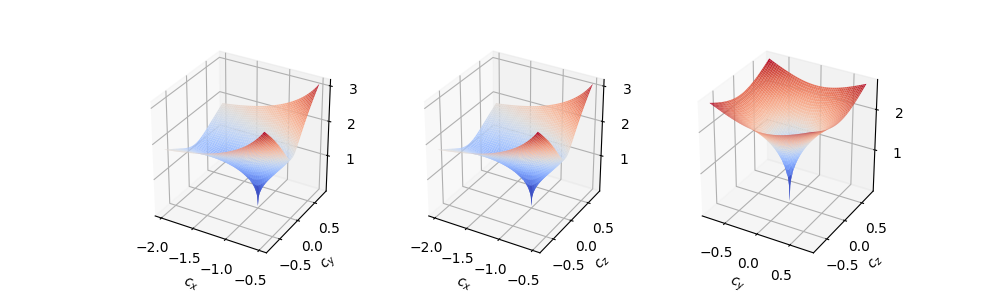
\includegraphics[width=\linewidth]{figures/gradient-xyz.png}
  \caption{Behavior of objective function on $c_x$-$c_y$, $c_x$-$c_z$ and $c_y$-$c_z$ planes.}
  \label{fig:gradient-xyz}
\end{figure}

\begin{figure}[h]
  \centering
  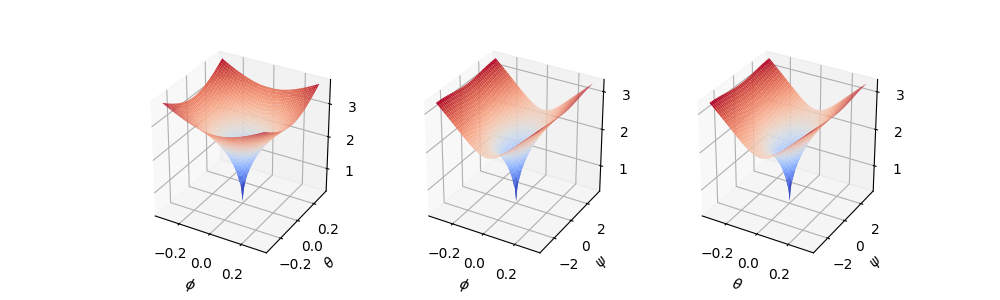
\includegraphics[width=\linewidth]{figures/gradient-angles.png}
  \caption{Behavior of objective function on $\phi$-$\theta$, $\phi$-$\psi$ and $\theta$-$\psi$ planes.}
  \label{fig:gradient-angles}
\end{figure}

From our crude investigation it appears that the objective function is differentiable and has no other local minima besides $\bomega^\dagger$
in its neighborhood or saddle points.
So we will try gradient descent methods first.

\subsection{Follow the gradient}
The simplest gradient descent iteration is
\begin{equation}
  \bomega_{k+1} = \bomega_{k} - a_k \nabla \mathcal{S}\left(\bomega_{k}\right)\text{,}
\end{equation}
where $\bomega_k$ is the estimate of the unknown parameter and $a_k$ is the step size at the $k$-th step.
The step size is determined as
\begin{equation}
  a_k = \frac{\vec{g}_k^\mathrm{T} \vec{g}_k}{\vec{g}_k^\mathrm{T} \vec{H}_k \vec{g}_k}\text{,}
\end{equation}
where $\vec{g}_k$ and $\vec{H}_k$ are the gradient $\nabla\mathcal{S}$ and Hessian $\nabla^2\mathcal{S}$ at the $k$-th step.
Such step size minimises the objective function along the direction of its gradient, since
\begin{equation*}
  \begin{split}
    \mathcal{S}\left(\bomega_{k+1}\right) = & \mathcal{S}\left(\bomega_k\right) + \nabla\mathcal{S}\left(\bomega_k\right)^\mathrm{T} \left(\bomega_{k+1}-\bomega_k\right) + \left(\bomega_{k+1}-\bomega_k\right)^\mathrm{T} \nabla^2\mathcal{S}\left(\bomega_k\right) \left(\bomega_{k+1}-\bomega_k\right) + \cdots \\
    \approx & \mathcal{S}\left(\bomega_k\right) + a_k \vec{g}_k^\mathrm{T} \vec{g}_k + \frac{a_k^2}{2}\vec{g}_k^\mathrm{T} \vec{H}_k \vec{g}_k \implies \\
    \frac{\partial \mathcal{S}\left(\bomega_{k+1}\right)}{\partial a_k} = & \vec{g}_k^\mathrm{T}\vec{g}_k + a_k \vec{g}_k^\mathrm{T} \vec{H}_k \vec{g}_k \text{.}
  \end{split}
\end{equation*}

With above approach soon we discovered our earlier investigation on the behavior of the objective function was far from the truth --
there are local minima nearly everywhere near the solution!

We have tried to escape from saddle points as well as undesired local minima with adaptive step size, random initial estimate and perturbations.
Although techniques help gradient descent method escape from saddle point exist,
however, such techniques still require extra iterations \citep{jin2017escape}.
Next we will try other approaches and perhaps come back to this topic later.

\subsection{Strike while the iron is hot}

\section{Perspective transform}

\bibliographystyle{plainnat}
\bibliography{main}
\end{document}
